\documentclass{article}
\usepackage[UTF8]{ctex} % 支持中文
\usepackage{graphicx} % 必须引入graphicx宏包以支持\includegraphics

\title{LaTeX图表练习}
\author{刘浩洋 24040021022}
\date{2025年8月31日}

\begin{document}

\maketitle

% --- 插入图片 ---
\section{插入图片}
使用 \texttt{graphicx} 宏包的 \texttt{\textbackslash includegraphics} 命令可以插入图片。图片文件(如PNG, JPG, PDF)需与.tex文件在同一目录下。

\begin{figure}[htbp]
    \centering % 将图片居中显示
    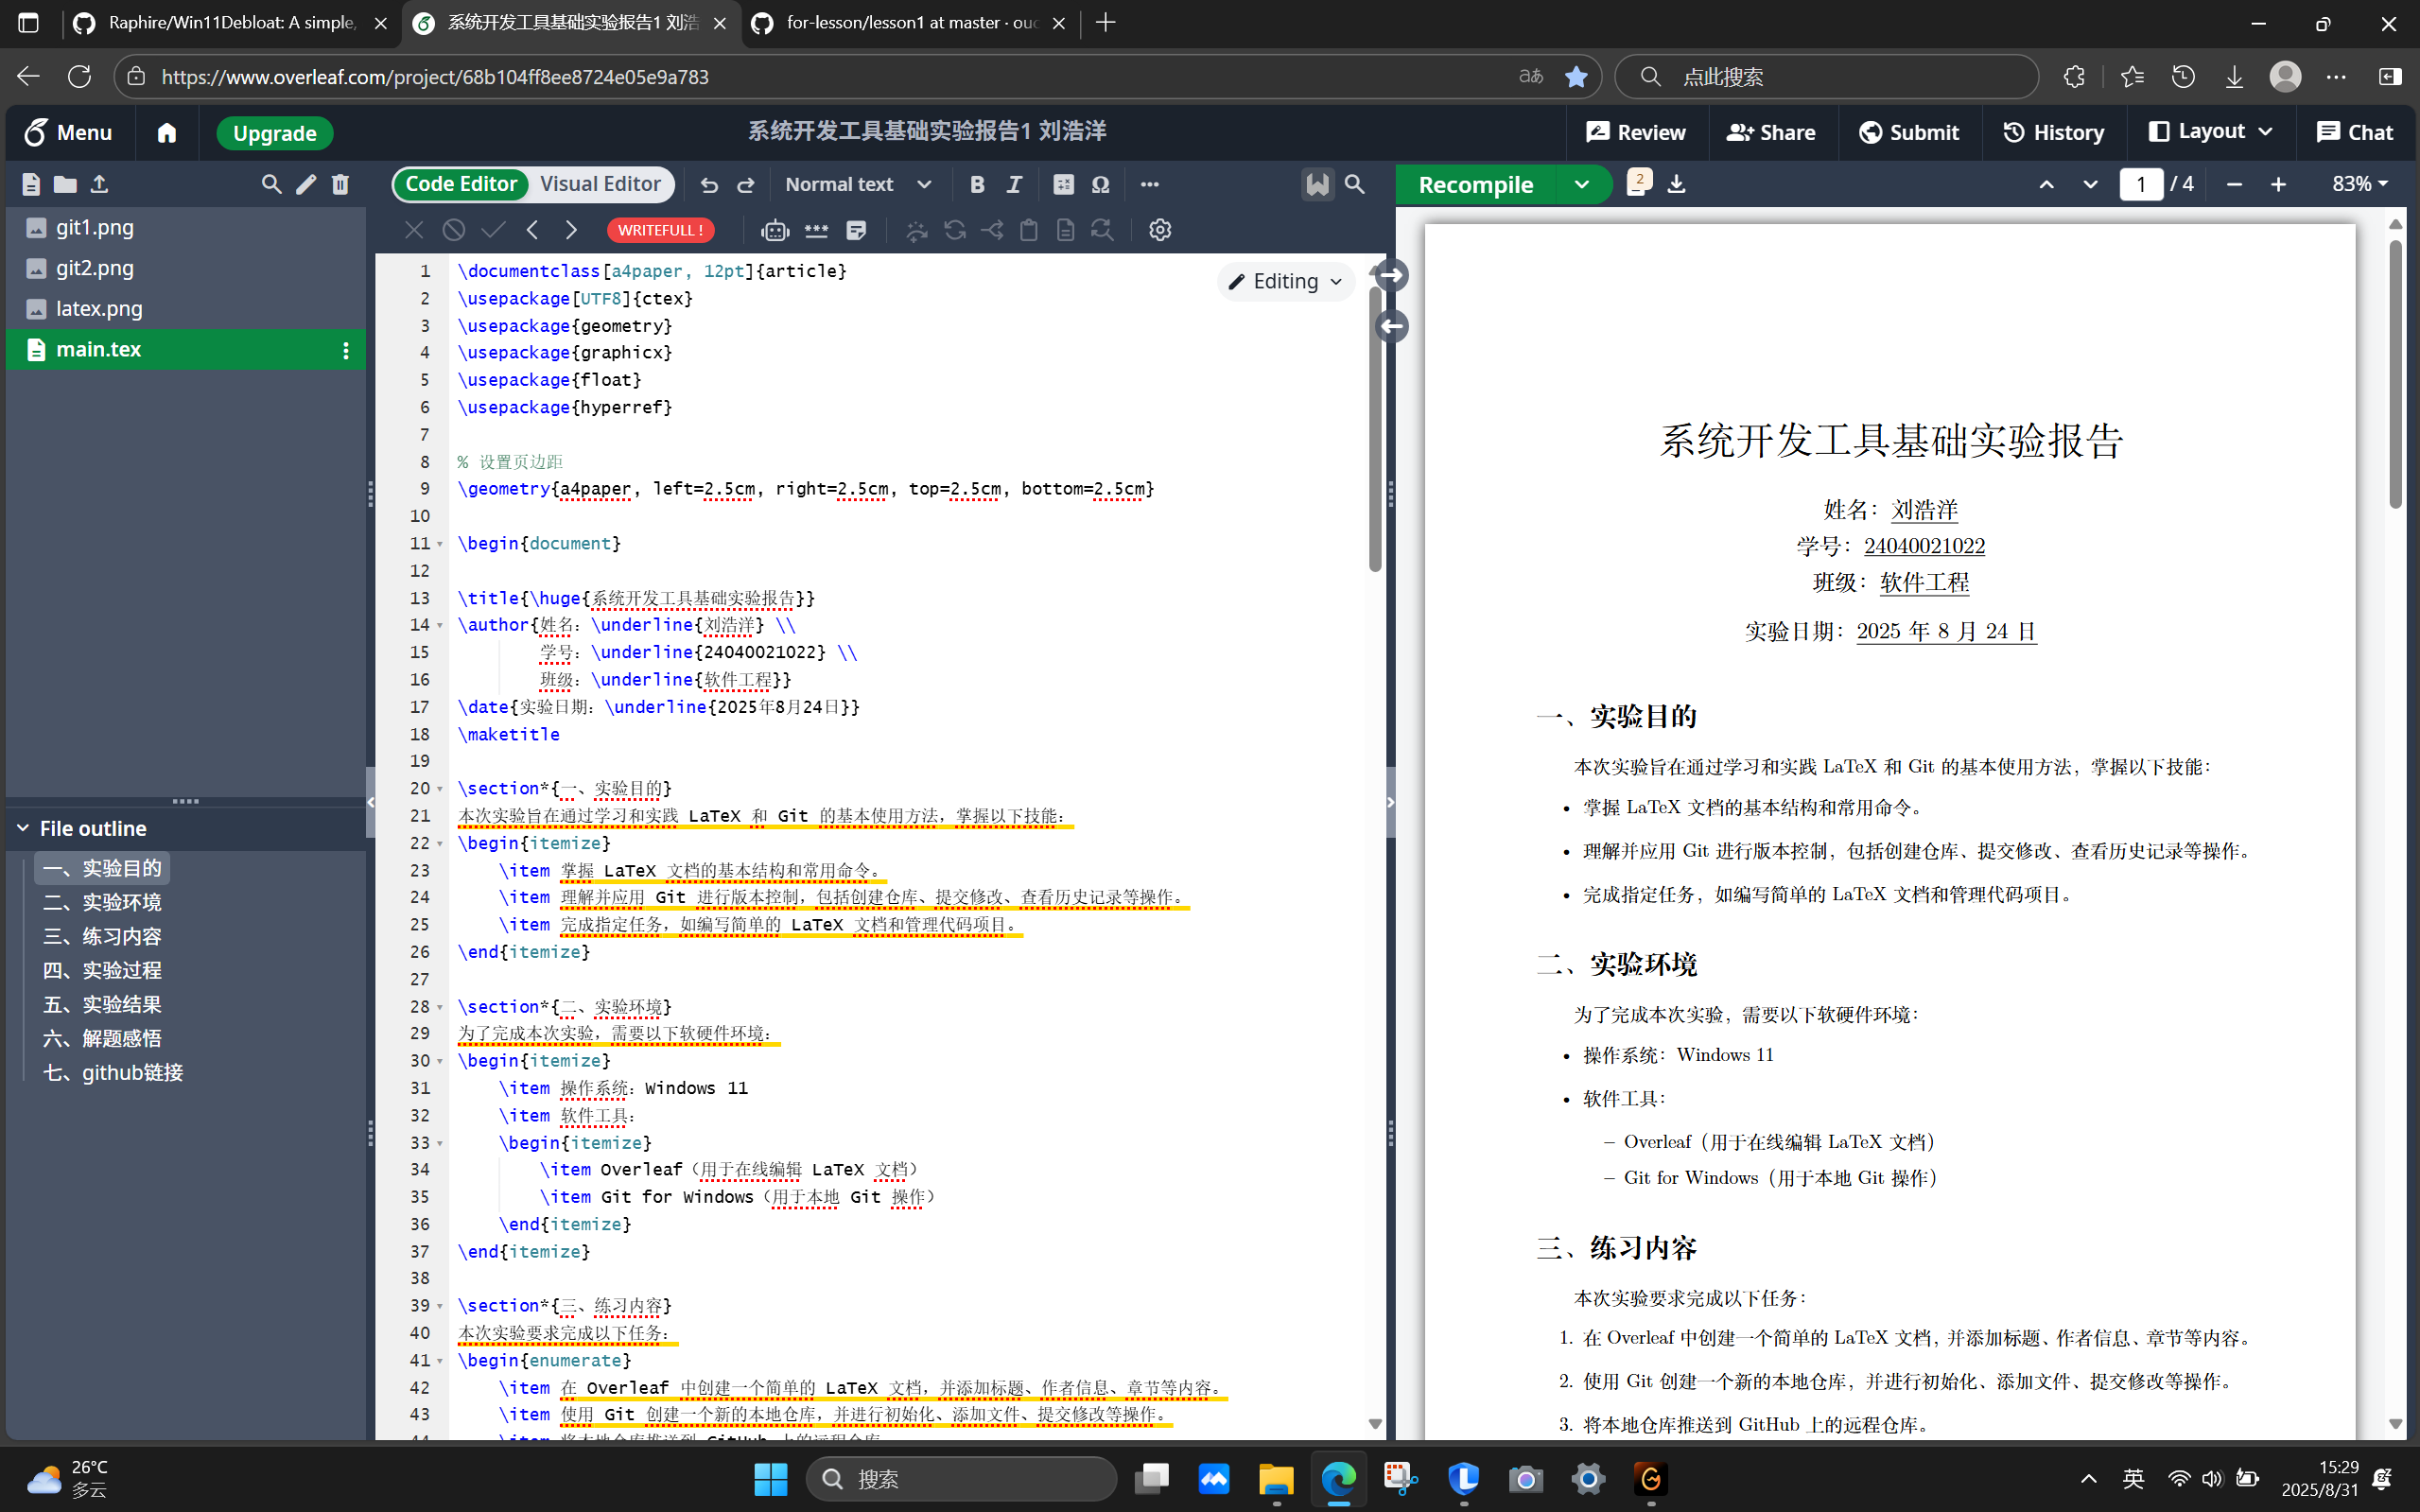
\includegraphics[width=0.6\textwidth]{example-image.png} % 设置图片宽度为文本宽度的60%
    \caption{这是一个示例图片。展示了如何在LaTeX中插入和调整图片。}
    \label{fig:example}
\end{figure}

% --- 不同尺寸的图片 ---
\section{调整图片尺寸}
可以通过 \texttt{width} 或 \texttt{scale} 参数调整图片大小。

\begin{figure}[h]
    \centering
    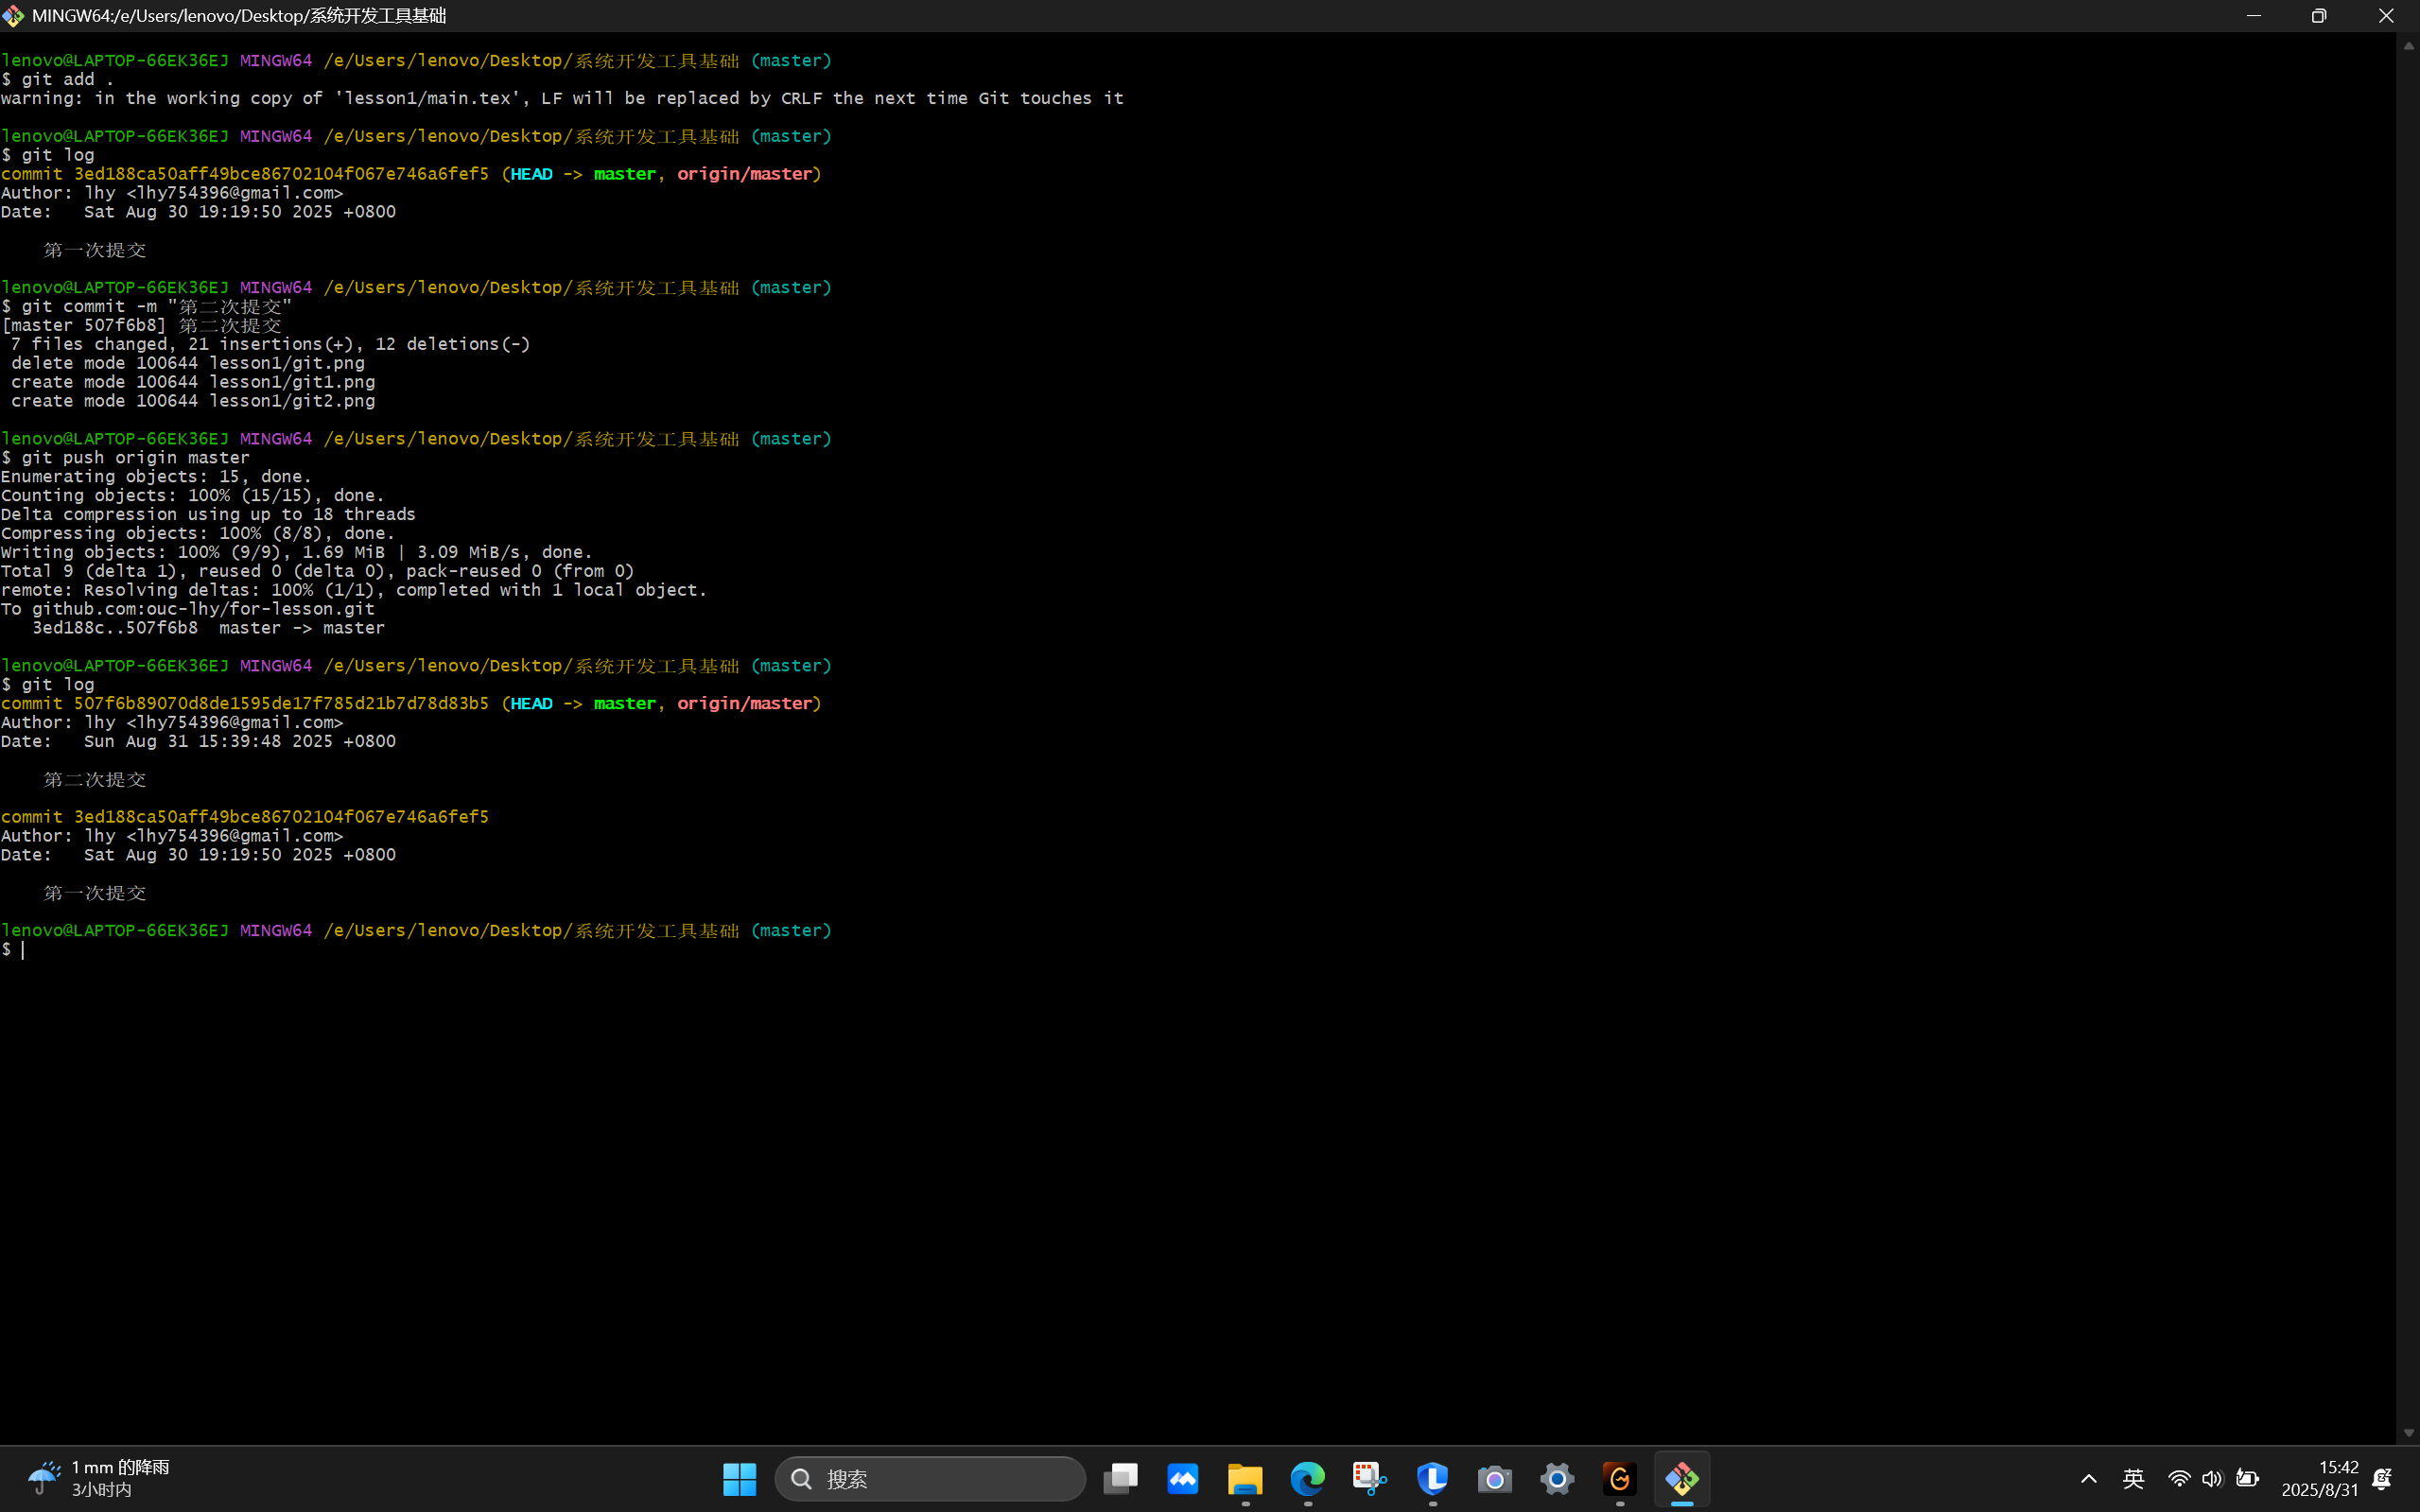
\includegraphics[width=3cm]{example-image-a.png} % 按指定宽度缩放
    \caption{指定宽度为3厘米的图片。}
    \label{fig:width}
\end{figure}

\begin{figure}[h]
    \centering
    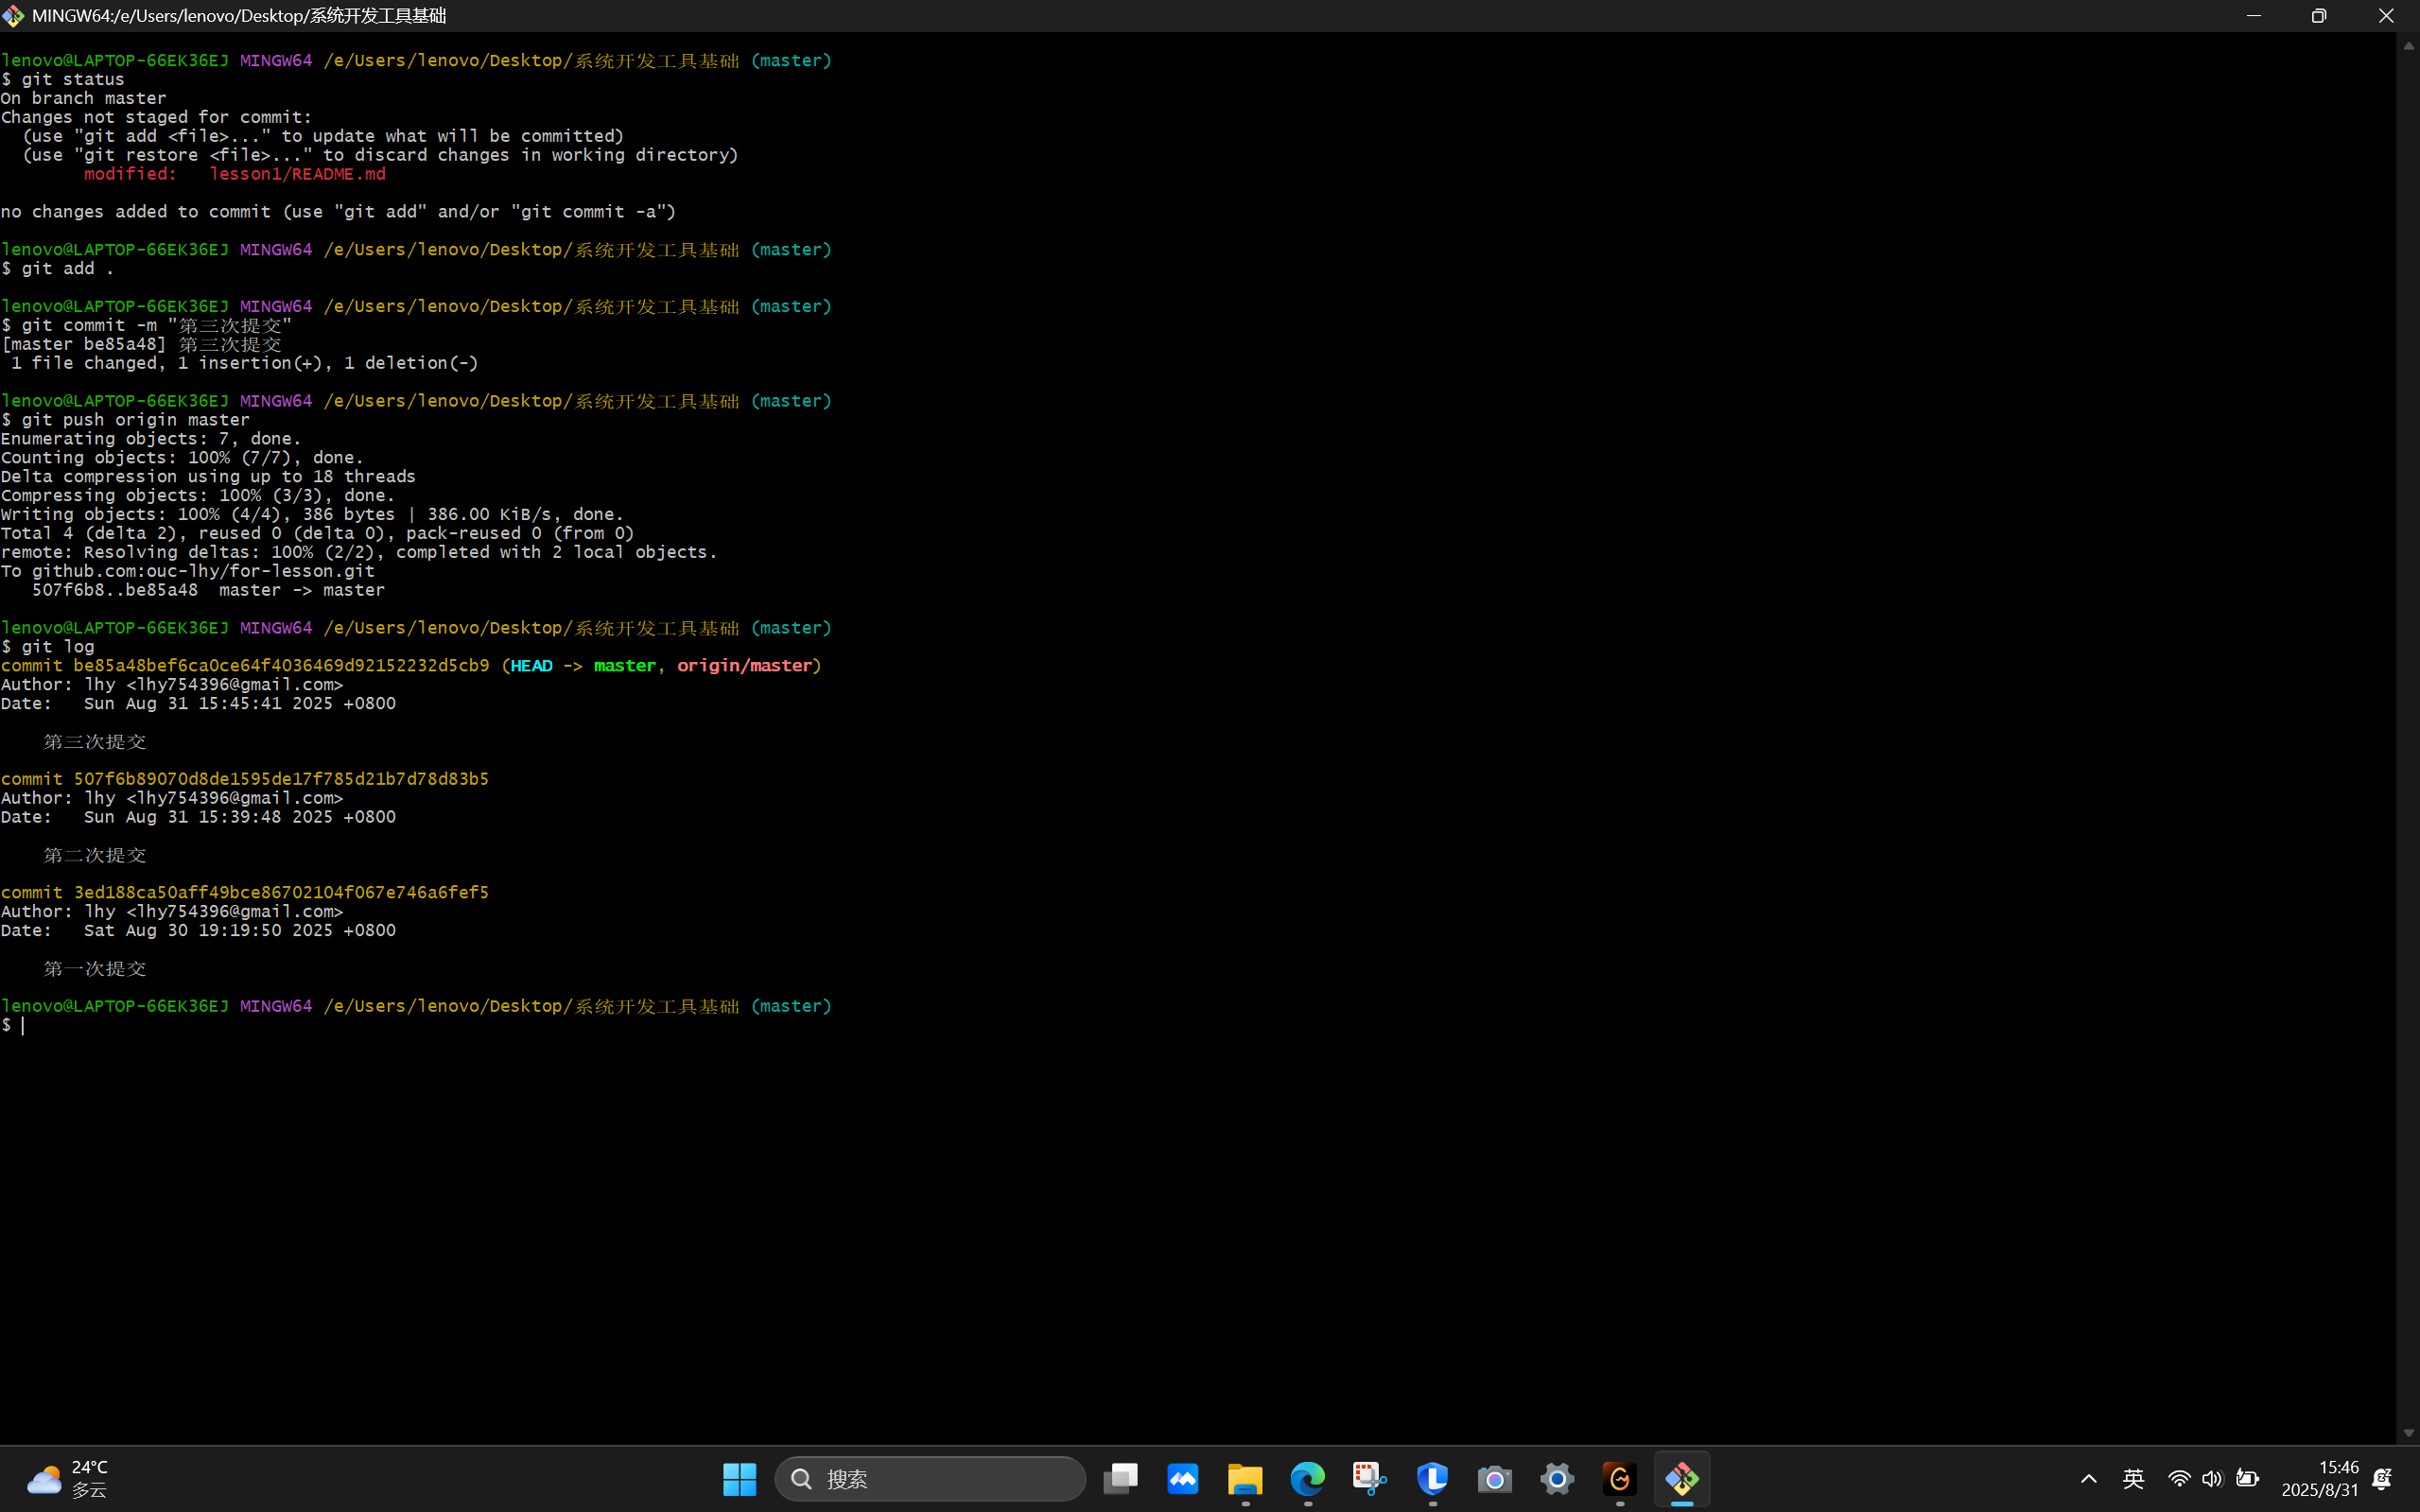
\includegraphics[scale=0.1]{example-image-b.png} % 按比例缩放(缩小到30%)
    \caption{按比例缩小到10\%的图片。}
    \label{fig:scale}
\end{figure}

% --- 在正文中引用图表 ---
\section{引用图表}
在正文中可以通过 \texttt{\textbackslash ref\{...\}} 引用图表的编号。例如,如图 \ref{fig:example} 所示,我们成功插入了一张图片。图 \ref{fig:width} 展示了如何精确控制图片宽度,而图 \ref{fig:scale} 则使用了比例缩放。

% --- 说明 ---
% 位置参数说明:
% h: here (当前位置附近)
% t: top (页面顶部)
% b: bottom (页面底部)
% p: page (单独一页)
% !: 强制LaTeX尽可能满足位置要求(如 [h!])

\end{document}